\chapter{Výsledky}

Detekce příjmu karbohydrátů a fyzické aktivity je testována na testovacích datech datasetu BGLP.

Pravdivě pozitivní detekce (TP) jsou hodnoty, kdy je aktivita (příjem jídla nebo fyzická aktivita) detekována (hodnota detekce alespoň 1) do dvou hodin od jejího zadání pacientem. Pokud je hodnota detekce 2, je aktivita brána jako potvrzená. Pakliže aktivita není detekována do dvou hodin od zadání, je výsledek falešně negativní (FN). V případě detekce hodnoty 2, kdy aktivita není zadaná, je výsledek falešně pozitvní (FP). Zároveň je počítáno zpoždění detekce od zadání aktivity pacientem. Zárověň je možné nastavit minimální počet referenčních signálů za den, aby byla statistika daného dne zaznamenána do celkových výsledků měření.

Je spočítaná citlivost detekce (TPR), neboli míra pravdivě pozitivních detekcí vůči celkovému počtu zaznamenaných referenčních hodnot. Přesnost (PPV) je poměr pravdivě pozitivních detekcí vůči celkovému počtu detekcí. FNR je míra falešně negativních výsledků vůči celkovému počtu zaznamenaných referenčních hodnot. FDR je míra falešně pozitivních výsledků vůči celkovému počtu detekcí. Dále je spočteno F1 skóre, které udává harmonický průměr citlivosti a přesnosti. F1 skóre se spočítá jako:

\scalebox{1.2}{$F_{1}=2*\frac{PPV*TPR}{PPV+TPR}$}

Počet pravdivě negativních výsledků nelze spolehlivě určit, protože změny v měřených datech přetrvávají i po ukončení aktivity. Proto není ani možné spočítat specificitu.


\section{Detekce karbohydrátů}

Algoritmy detekce karbohydrátů byly testovány na datech jedenácti pacientů. Měření testovacích dat u každého pacienta probíhalo po dobu 10 - 11 dnů. V součtu pacienti zaznamenali 340 jídel za 109 dnů. Diabetičtí pacienti musí pravidelně jíst (uvádí se 5-6x denně). Proto se statistika z každého dne zaznamená byli-li zadány alespoň 3 jídla. V opačném případě je vysoká pravděpodobnost, pacient některé jídlo nezaznamenal, což by ovlivnilo výsledky.

Testované algoritmy jsou detekce hran průběhu intersticiální glukózy, kdy potvrzení je nastaveným vyšším thresholdem nebo rekurentní neuronovou sítí, a samostatná GRU neuronová síť.

V tabulkách \ref{tab:vys:th} až \ref{tab:vys:thrnn} v příloze A jsou výsledky detekce pro jednotlivé pacienty. V tabulce \ref{tab:res_cho} jsou průměrné výsledky.

\begin{table}[H]
\caption{Výsledky detekce karbohydrátů}
\label{tab:res_cho}
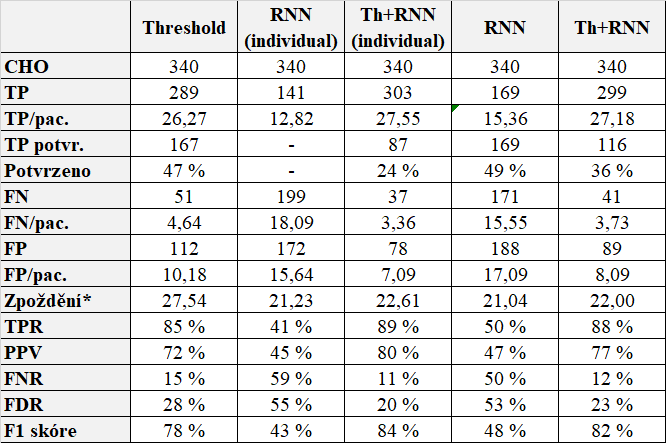
\includegraphics[width=1\textwidth]{img/vysledky/cho/cho.png}
\begin{flushleft}
* průměrná doba detekce karbohydrátů od příjetí jídla v minutách\\
\begin{tabular}{ll}
CHO & - počet zaznamenaných jídel\\
TP & - pravdivě pozitivní\\
FN & - falešně negativní\\
FP & - falešně pozitivní\\
TPR & - citlivost - míra pravdivě pozitivních\\
PPV & - přesnost\\
FNR & - míra falešně negativních výsledků \\
FDR & - míra falešně pozitivních výsledků\\
\end{tabular}
\end{flushleft}
\end{table}
\vspace*{-7mm}

Všechny formy detekce hran průběhu intersticiální glukózy dosahovali citlivosti nad 85 \%. Nejlepších výsledků dosahuje detekce hran s potvrzením GRU neuronovou sítí. U některých pacientů dosahovala citlivost až 95 \%. Tato metoda má i nejnižší počet falešně pozitivních detekcí. Naopak samostatná neuronová síť dosahovala úspěšné detekce jen kolem 50 \%.

Zpoždění v průměru 22 minut je srovnatelné, nebo i lepší, než výsledky zkoumaných algoritmů v kapitole \ref{ch:analyzaCHO}.

Algoritmy vykazují značný počet falešně pozitivních detekcí. To může být dáno častými výkyvy glukózy u pacienta nebo tím, že pacienti jídlo nezadávali poctivě, nebo ho zadali se zpožděním. Také prudké výkyvy koncentrace cukru v krvi spojené s jinou činností mohou způsobit falešnou detekci.

V grafu na obrázku \ref{fig:res_cho} je porovnání jednotlivých metod.

\begin{figure}[H]
\caption{Porovnání metod detekce karbohydrátů}
\label{fig:res_cho}
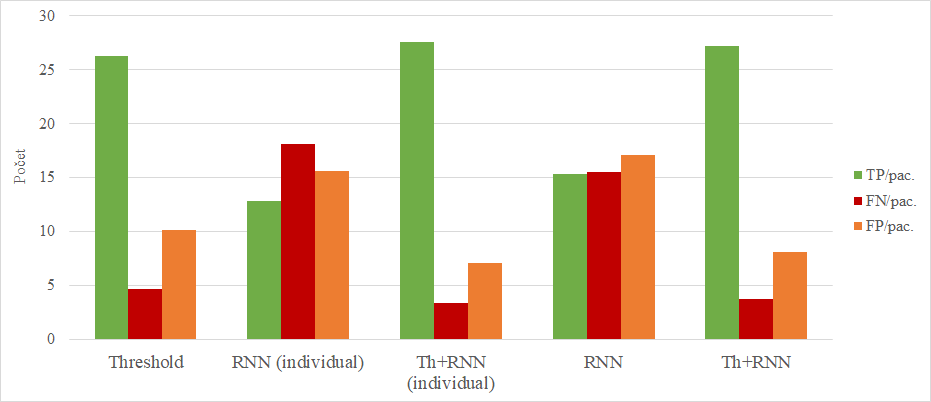
\includegraphics[width=1\textwidth]{img/vysledky/cho/tp.png}
\end{figure}


\section{Detekce fyzické aktivity}

Pro detekci fyzické aktivity jsou použity hodnoty srdečního tepy, počtu kroků, akcelerace, elektrodermální aktivity a jejich kombinace. Thresholdy jsou různé pro každý ukazatel a pacienta. Threshold pro srdeční tep se pohybuje od 100 do 120 tepů za minutu, počet kroků od 12 do 45 za 5 minut, velikost akcelerace od 1,1 do 1,5 $m/s_{2}$ a elektrodermální aktivita od 1 do 15 siemensů.

Pět pacientů mělo měřen srdeční tep, počet kroků a elektrodermální aktivitu. Čtyři pacienti měli měřenou akceleraci a elektrodermální aktivitu. Pro tři pacienty nejsou dostupná testovací data se zadanou fyzickou aktivitou, proto nebyly zařazeni do testů.

V tabulkách \ref{tab:vys:heart} až \ref{tab:vys:steps+} v příloze A jsou výsledky detekce u pacientů s měřeným srdečním tepem. V tabulkách \ref{tab:vys:acc} až \ref{tab:vys:acc+} jsou výsledky detekce u pacientů s měřenou akcelerací. V tabulkách jsou i velikosti nastavených thresholdů pro jednotlivé ukazatele. V tabulce \ref{tab:res_heart} jsou souhrnné výsledky pro srdeční tep a počet kroků, v tabulce \ref{tab:res_acc} pro akceleraci.

\begin{table}[H]
\caption{Výsledky detekce fyzické aktivity\\ - srdeční tep, počet kroků, elektrodermální aktivita}
\label{tab:res_heart}
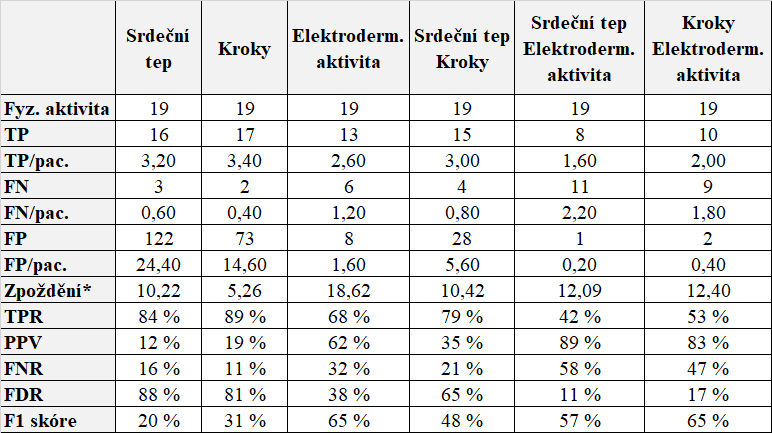
\includegraphics[width=1\textwidth]{img/vysledky/pa/vysledky 1.png}
\end{table}

\begin{table}[H]
\caption{Výsledky detekce fyzické aktivity\\ - akcelerace, elektrodermální aktivita}
\label{tab:res_acc}
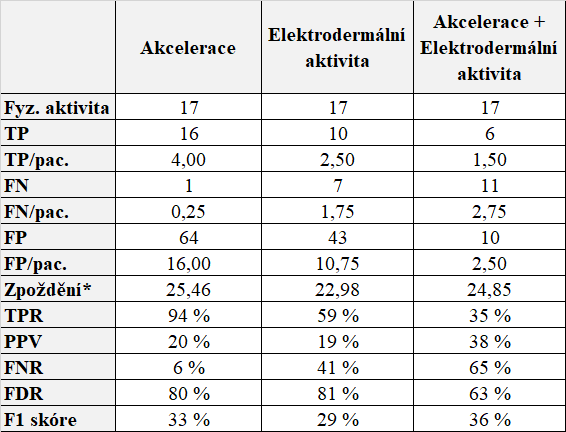
\includegraphics[width=0.8\textwidth]{img/vysledky/pa/vysledky 2.png}
\end{table}

Dobré citlivosti dosahovala detekce při použití srdečního tepu, kroků a akcelerace, přičemž akcelerace dosahovala citlivosti 94 \%. Nejnižší zpoždění mělo měření počtu kroků. Nejmenší citlivost má elektrodermální aktivita.

Všechny algoritmy mají vysoký počet falešně pozitivních detekcí. To je dáno tím, že měřená data jsou ovlivněna mnoha faktory, které nemusí s intenzivní fyzickou aktivitou souviset. Může se také jednat o lehčí aktivitu, kterou pacient nezadal. Kombinací více ukazatelů se podařilo značně snížit počet falešně pozitivních detekcí. nejlépe pak vychází kombinace srdečního tepu a počtu kroků.

Detekce sestupné hrany neměla vliv na výsledky detekcí. Z toho vyplývá, že ve všech případech, kdy byla fyzická aktivita detekována hodnota intersticiální glukózy klesala.

V grafech na obrázcích \ref{fig:res_heart} a \ref{fig:res_acc} je porovnání jednotlivých metod.

\begin{figure}[H]
\caption{Porovnání metod detekce fyzické aktivity\\ - srdeční tep, počet kroků, elektrodermální aktivita}
\label{fig:res_heart}
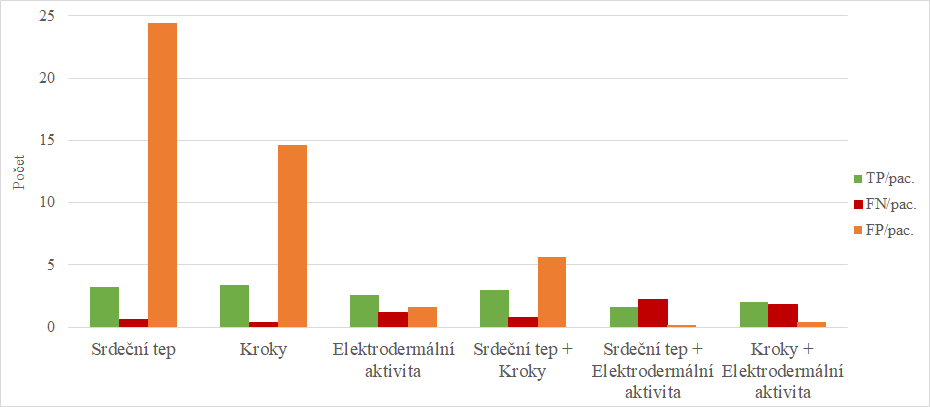
\includegraphics[width=1\textwidth]{img/vysledky/pa/g1.png}
\end{figure}

\begin{figure}[H]
\caption{Porovnání metod detekce fyzické aktivity\\ - akcelerace, elektrodermální aktivita}
\label{fig:res_acc}
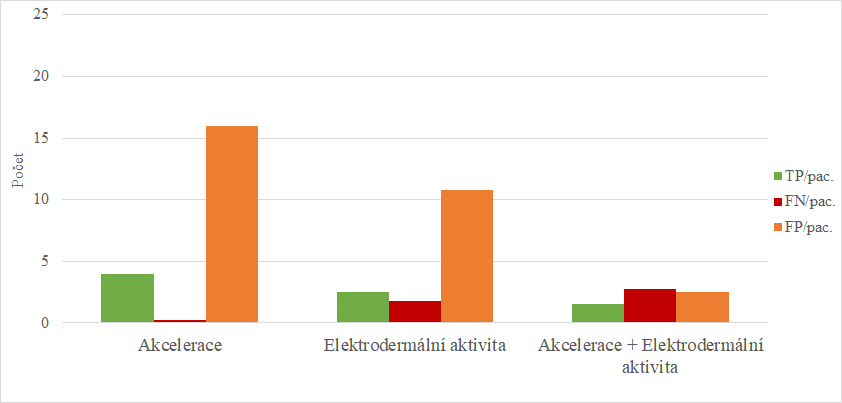
\includegraphics[width=1\textwidth]{img/vysledky/pa/g2.png}
\end{figure}